\documentclass[aspectratio=169,11pt,hyperref={colorlinks=true}]{beamer}
\usepackage[utf8]{inputenc}
\usepackage[T1]{fontenc}
\usepackage{fontspec}
\usepackage[absolute,overlay]{textpos}
% Code snippits
\usepackage{listingsutf8}
\usepackage{listings-golang}
\usepackage{listings}
\usepackage{tikz}
\usepackage{color}
\setbeamertemplate{navigation symbols}{}
\definecolor{ibm}{RGB}{70,107,176}
\definecolor{mainfg}{RGB}{0,0,0}
\setbeamercolor{titlelike}{fg=mainfg}
\setbeamercolor{structure}{fg=mainfg}
% \hypersetup{colorlinks,urlcolor=mainfg}
\setbeamertemplate{footline}[frame number]
% \RequirePackage{animate subfigure media9 ocgx2 pgfplots}
% run the following command to install package:
% sudo tlmgr install animate subfigure media9 ocgx2 pgfplots
% Inserting graphics
\usepackage{graphicx}
% Side-by-side figures, etc
\usepackage{subfigure}
\usepackage{amsmath}
\usepackage{tikz}
\usepackage{tipa}
\newcommand{\light}[1]{\textcolor{gray}{#1}}
\usepackage{hyperref}
\usepackage{animate}
\usepackage{pgfplots}
\pgfplotsset{compat=1.16}
\usepackage{pgfplotstable}
\usepackage{colortbl}
\usepackage{booktabs}

\definecolor{mygreen}{rgb}{0,0.6,0}
\definecolor{mygray}{rgb}{0.5,0.5,0.5}
\definecolor{mymauve}{rgb}{0.58,0,0.82}

\pgfplotstableset{col sep=comma, header=has colnames}

\lstset{ %
  backgroundcolor=\color{white},   % choose the background color; you must add \usepackage{color} or \usepackage{xcolor}
  breakatwhitespace=false,         % sets if automatic breaks should only happen at whitespace
  breaklines=true,                 % sets automatic line breaking
  captionpos=b,                    % sets the caption-position to bottom
  commentstyle=\color{mainfg},        % comment style
  extendedchars=true,              % lets you use non-ASCII characters; for 8-bits encodings only, does not work with UTF-8
  keepspaces=true,                 % keeps spaces in text, useful for keeping indentation of code (possibly needs columns=flexible)
  keywordstyle=\color{blue},       % keyword style
  otherkeywords={*,...},           % if you want to add more keywords to the set
  numbersep=5pt,                   % how far the line-numbers are from the code
  numberstyle=\tiny\color{mygray}, % the style that is used for the line-numbers
  rulecolor=\color{black},         % if not set, the frame-color may be changed on line-breaks within not-black text (e.g. comments (green here))
  showspaces=false,                % show spaces everywhere adding particular underscores; it overrides 'showstringspaces'
  showstringspaces=false,          % underline spaces within strings only
  showtabs=false,                  % show tabs within strings adding particular underscores
  stringstyle=\color{mainfg},         % string literal style
}

\setbeamerfont{caption}{series=\normalfont,size=\fontsize{8}{10}}
\setbeamertemplate{caption}{\raggedright\insertcaption\par}

\setlength{\abovecaptionskip}{0pt}
\setlength{\floatsep}{0pt}

% TBD space between authors
\author[Kyra Matt Andrea]{%
\normalsize Kyra Wulffert \tiny kwulffert@gmail.com \\
\normalsize Matthew Treinish \tiny mtreinish@kortar.org \\
\normalsize Andrea Frittoli \tiny andrea.frittoli@gmail.com \\
\normalsize
}

\date{November 22, 2019}
\title{Machine Learning for CI}
\institute[ODSC]{
  Open Data Science Conference \\
  London 2019
}

% \usetheme{ibmcloud}
% Themes: https://mpetroff.net/files/beamer-theme-matrix/
\usetheme{default}
\usecolortheme{crane}

\begin{document}

\begin{frame}[noframenumbering]
\titlepage{}
\end{frame}

\section{Context}

% TBD: Update the graph to a recent one
\begin{frame}
  \frametitle{CI at Scale}
  \begin{columns}
    \column{0.6\linewidth}
      \begin{figure}
      \begin{center}
        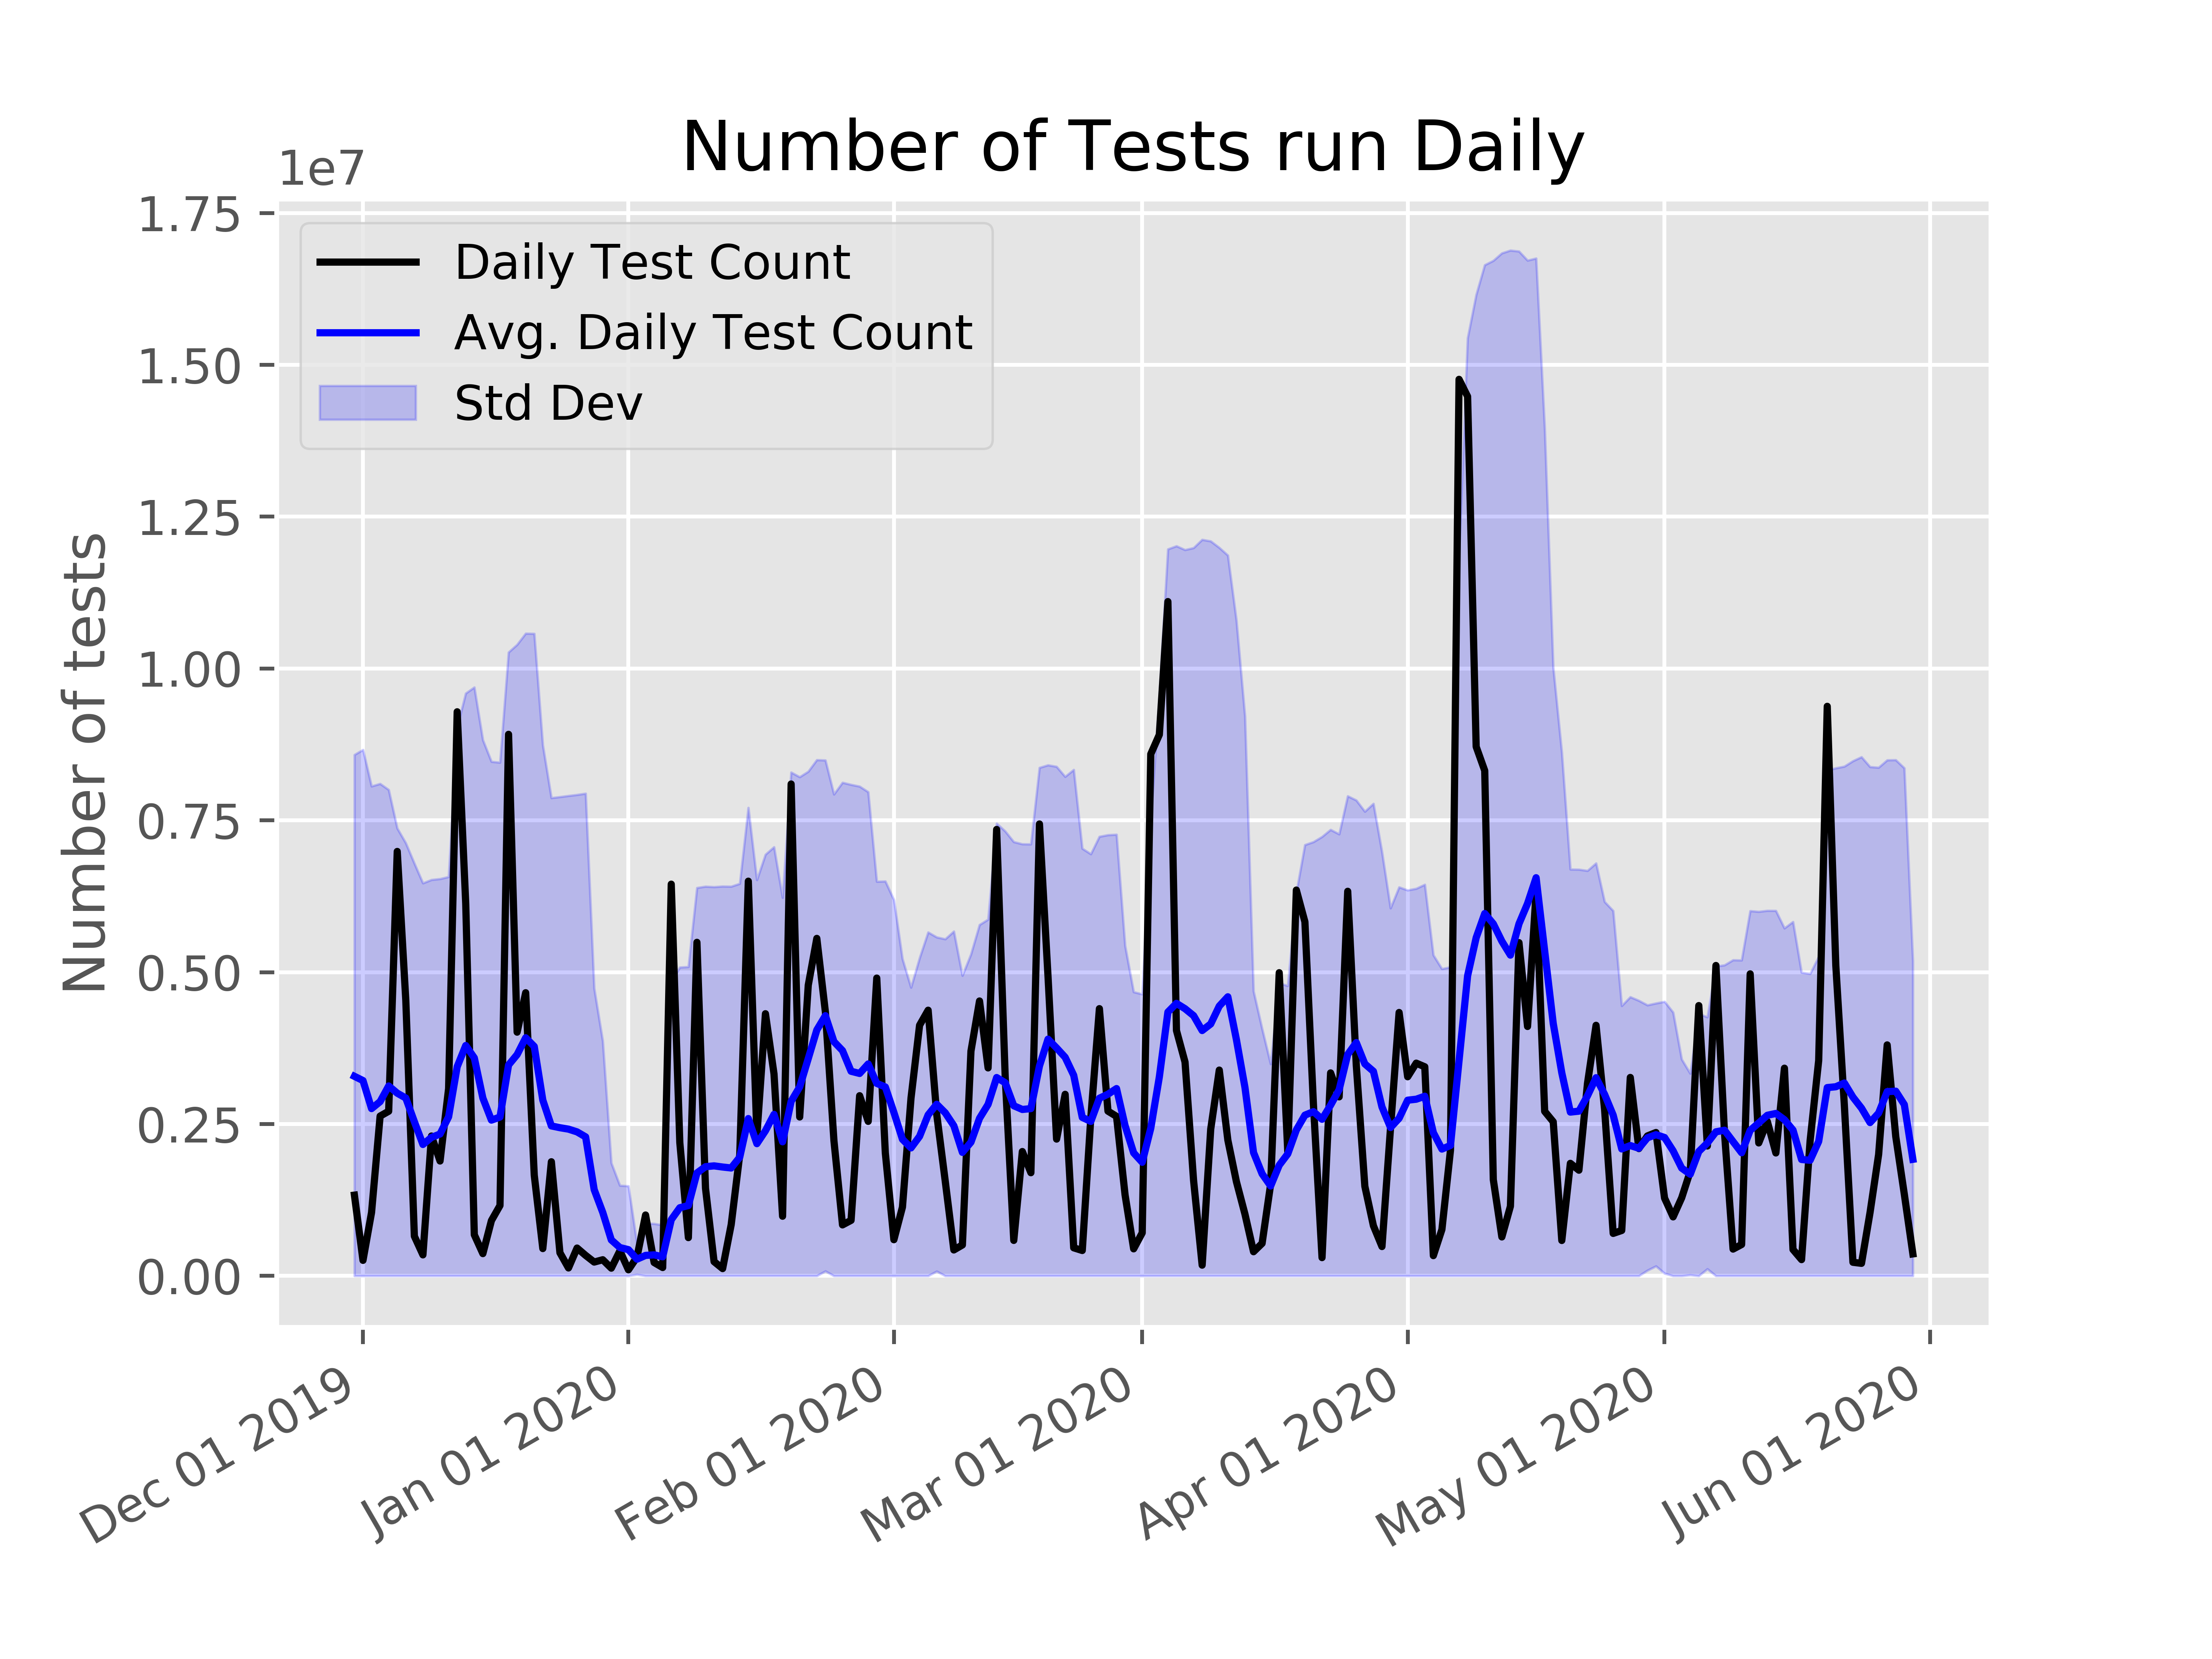
\includegraphics[width=0.9\textwidth]{graphs/daily_count.png}
           \caption{Source: subunit2sql-graph dailycount}
      \end{center}
      \end{figure}
    \column{0.4\linewidth}
      \begin{itemize}
          \item{Continuous Integration}
          \item{Continuous Log Data}
          \item{Lots of data, little time}
          \item{Triaging failures?}
          \item{AI to the rescue!}
      \end{itemize}
  \end{columns}
\end{frame}

\begin{frame}
    \frametitle{The OpenStack use case}
    \begin{columns}
      \column{0.5\linewidth}
        \begin{itemize}
            \item{Integration testing in a VM}
            \item{System logs, application logs}
            \item{Dstat data}
            \item{Gate testing}
            \item{Not only OpenStack}
        \end{itemize}
      % Add a picture with dstat graph samples
      \column{0.5\linewidth}
        \begin{figure}
        \begin{center}
          \animategraphics[autoplay,width=0.8\linewidth]{1}{graphs/100norm/1min_normalized_}{0}{99}
            \caption{Normalized system average load for different examples}
        \end{center}
        \end{figure}
    \end{columns}
\end{frame}

\section{Infrastructure}
\begin{frame}
    \frametitle{Collecting data}
    \begin{columns}
      \column{0.5\linewidth}
        \begin{figure}
        \begin{center}
          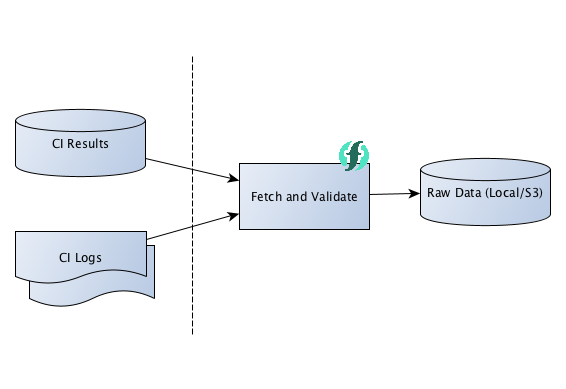
\includegraphics[width=1\textwidth]{diagrams/cache-data.png}
             \caption{Data caching diagram}
        \end{center}
        \end{figure}
      \column{0.5\linewidth}
        \begin{itemize}
            \item{Automation and repeatability}
            \item{Light-weight data validation}
            \item{Object storage for data}
            \item{Periodic Action on OpenWhisk}
        \end{itemize}
    \end{columns}
\end{frame}

\begin{frame}
    \frametitle{Experiment Workflow}
    % TBD Add comment on Tekton / logo
    \begin{columns}
      \column{0.4\linewidth}
        \begin{itemize}
            \item{\textbf{Visualize data}}
            \item{\textbf{Define a dataset}}
            \item{Define an experiment}
            \item{Run the training}
            \item{Collect results}
            % TBD twice? Change to review or ~
            \item{Visualize data}
        \end{itemize}
        \column{0.6\linewidth}
          \begin{figure}
            \lstinputlisting[basicstyle=\tiny,language=bash]{code/define_dataset.sh}
          \end{figure}
          \begin{figure}
            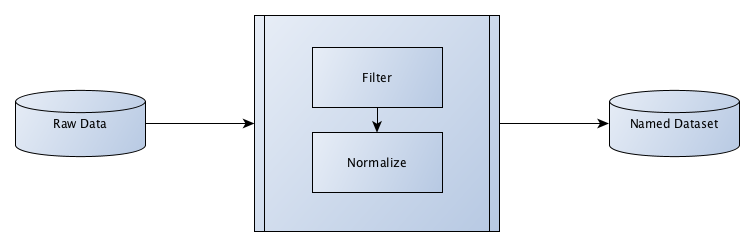
\includegraphics[width=1\textwidth]{diagrams/build-dataset.png}
            \caption{Dataset preparation diagram}
          \end{figure}
    \end{columns}
\end{frame}

\subsection{Data}
\begin{frame}
    \frametitle{Data Selection}
    \begin{columns}
      \column{0.5\linewidth}
        \begin{itemize}
            \item{What is dstat data?}
            \item{Experiment reproducibility}
            \item{Dataset selection}
            \begin{itemize}
              \item{Dstat feature selection}
              \item{Data resolution (down-sampling)}
            \end{itemize}
        \end{itemize}
      \column{0.5\linewidth}
      \begin{table}[h!]
        \begin{center}
          \caption{Sample of dstat data}
          \label{dstat_sample}
          \resizebox{0.7\linewidth}{!}{
            \pgfplotstabletypeset[
              columns/time/.style={string type},
              every head row/.style={after row=\midrule},
              every first row/.style={before row=\rowcolor{mygray}},
              every nth row={5}{before row=\rowcolor{mygray}},
              columns/usr/.style={column type/.add={>{\columncolor[gray]{.8}}}{}},
              columns/1m/.style={column type/.add={>{\columncolor[gray]{.8}}}{}},
            ]{code/dstat_sample.csv}
          }
        \end{center}
     \end{table}
  \end{columns}
\end{frame}

\begin{frame}
    \frametitle{Data Normalization}
    \begin{columns}
      \column{0.5\linewidth}
        \begin{itemize}
            \item{Unrolling}
            % (formula) x - mean / xmax - mmin
            % NOTE: each line in the unrolled table is a sample
        \end{itemize}
        \begin{table}[h!]
          \begin{center}
            \caption{Sample of unrolled data}
            \label{unrolled_sample}
            \resizebox{0.6\linewidth}{!}{
              \pgfplotstabletypeset[
                every head row/.style={after row=\midrule},
              ]{code/unrolled_sample.csv}
            }
          \end{center}
       \end{table}
      \column{0.5\linewidth}
      \begin{itemize}
          \item{Normalizing}
          % (formula) x - mean / xmax - xmin
      \end{itemize}
      \begin{table}[h!]
        \begin{center}
          \caption{Sample of normalized data}
          \label{normalized_sample}
          \resizebox{0.6\linewidth}{!}{
            \pgfplotstabletypeset[
              every head row/.style={after row=\midrule},
            ]{code/normalized_sample.csv}
          }
        \end{center}
     \end{table}
     \end{columns}
\end{frame}

\begin{frame}
    \frametitle{Building the dataset}
    % Dev is not used for dev, but for further evaluation and metrics report
    \begin{columns}
      \column{0.5\linewidth}
        \begin{figure}
        \begin{center}
          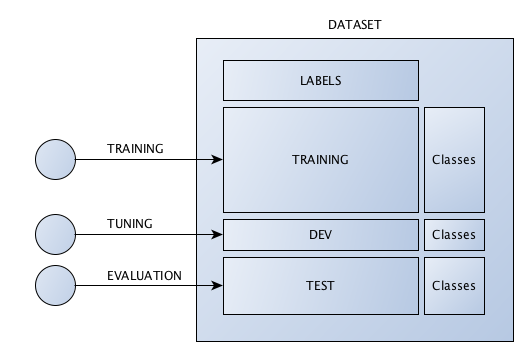
\includegraphics[width=0.9\textwidth]{diagrams/dataset.png}
             \caption{Structure of a dataset}
             % NOTE: the term "labels" is overloaded. In this case we mean the names of the features, like 'usr1', 'usr2' etc
        \end{center}
        \end{figure}
      \column{0.5\linewidth}
        \begin{itemize}
            \item{Split in training, dev, test}
            \item{Obtain classes}
            \item{Store normalized data on s3}
            \item{Input function for training}
            \item{Input function for evaluation}
        \end{itemize}
    \end{columns}
\end{frame}

% NOTE: check about "local" experiment, can we store it in S3 as well or not.
\begin{frame}
    \frametitle{Experiment Workflow}
    \begin{columns}
      \column{0.4\linewidth}
        \begin{itemize}
            \item{Visualize data}
            \item{Define a dataset}
            \item{\textbf{Define an experiment}}
            \item{\textbf{Run the training}}
            \item{\textbf{Collect results}}
            \item{Visualize data}
        \end{itemize}
        \column{0.6\linewidth}
          \begin{figure}
            \lstinputlisting[basicstyle=\tiny,language=bash]{code/define_experiment.sh}
          \end{figure}
          \begin{figure}
            % Replace ffdl with tekton
            \lstinputlisting[basicstyle=\tiny,language=bash]{code/run_training.sh}
          \end{figure}
    \end{columns}
\end{frame}

\begin{frame}
    \frametitle{Training Infrastructure}
    % Add tekton, details on kubeflow, open source
    \begin{columns}
      \column{0.5\linewidth}
        \begin{figure}
        \begin{center}
          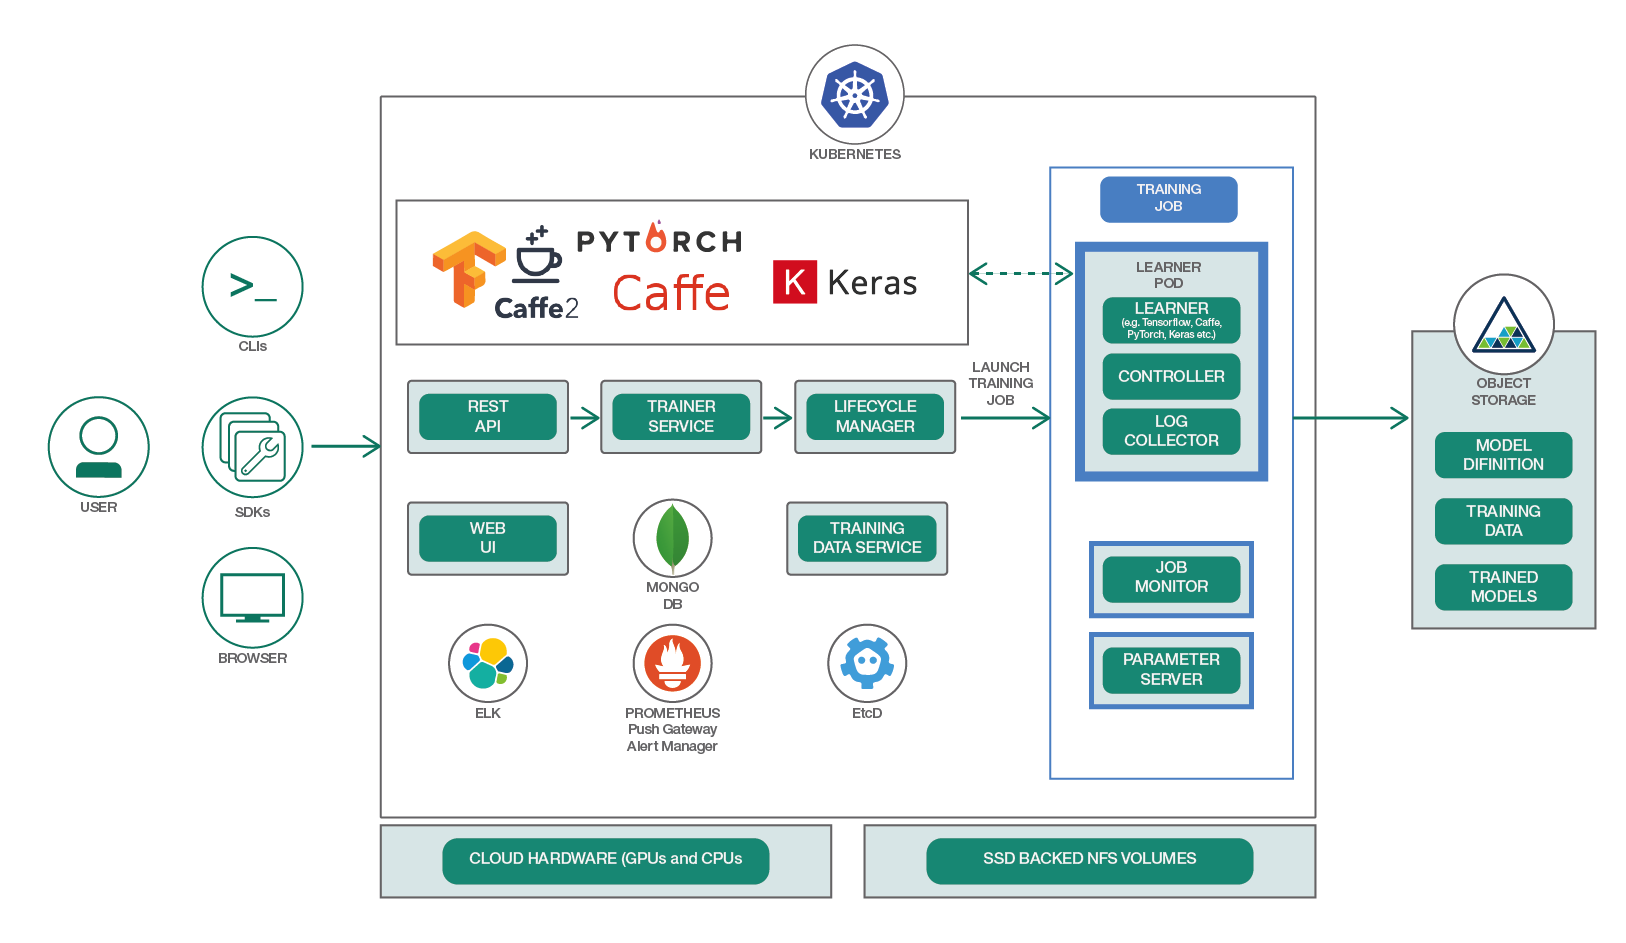
\includegraphics[width=1\textwidth]{diagrams/FfDL-Diagram.png}
             \caption{FfDL Architecture - Source: \href{https://developer.ibm.com/code/2018/03/20/democratize-ai-with-fabric-for-deep-learning/l}{https://developer.ibm.com/code/}}
        \end{center}
        \end{figure}
      \column{0.5\linewidth}
        \begin{itemize}
          \item{TensorFlow Estimator API}
          \item{CIML wrapper}
          \item{ML framework interchangable}
          \item{Training Options:}
          \begin{itemize}
            \item{Run on a local machine}
            \item{Helm deploy CIML, run in containers}
            \item{Submit training jobs to Ffdl}
            \item{\light{Kubeflow}}
          \end{itemize}
        \end{itemize}
    \end{columns}
\end{frame}

\begin{frame}
    \frametitle{Prediction}
    \begin{columns}
      \column{0.5\linewidth}
        \begin{itemize}
            \item{Event driven: near real time}
            \item{No request to serve the prediction to}
            \item{MQTT Trigger from the CI system}
            \item{CIML produces the prediction}
            \item{Trusted Source: Continuous Training}
        \end{itemize}
      \column{0.5\linewidth}
        \begin{itemize}
          \item{CIML kubernetes app components:}
          \begin{itemize}
            \item{MQTT Client receives events}
            \item{Data module fetches and prepares data}
            \item{TensorFlow wrapper issues the prediction}
            \item{Example: comment back on Gerrit/Github}
          \end{itemize}
        \end{itemize}
    \end{columns}
\end{frame}

\section{Experiments}
\begin{frame}
    \frametitle{DNN - Binary Classification}
    \begin{columns}
      \column{0.5\linewidth}
        \begin{itemize}
            \item{Classes: Passed or Failed}
            \item{Supervised training}
            \item{TensorFlow \emph{DNNClassifier}, classes=2}
            \item{Dataset:}
            \begin{itemize}
              \item{CI Job "tempest-full"}
              \item{Gate pipeline only}
              \item{3955 examples split in 60\% training, 20\% dev and 20\% test}
            \end{itemize}
            \item{Hyper-parameters:}
            \begin{itemize}
              \item{Activation function: ReLU}
              % ReLU: rectifier, non linear component of the neuron, standard for binary classification
              \item{Output layer: Sigmoid}
              % Best for binary classification 0,1
              \item{Optimizer: Adagrad}
              \item{Learning rate (initial): 0.05}
              \item{5 hidden layers, 100 units per layer}
              \item{Batch Size: 128, Epochs: 500}
              % Good practice for batch size is a power of 2
            \end{itemize}
        \end{itemize}
      \column{0.5\linewidth}
        \begin{figure}
        \begin{center}
          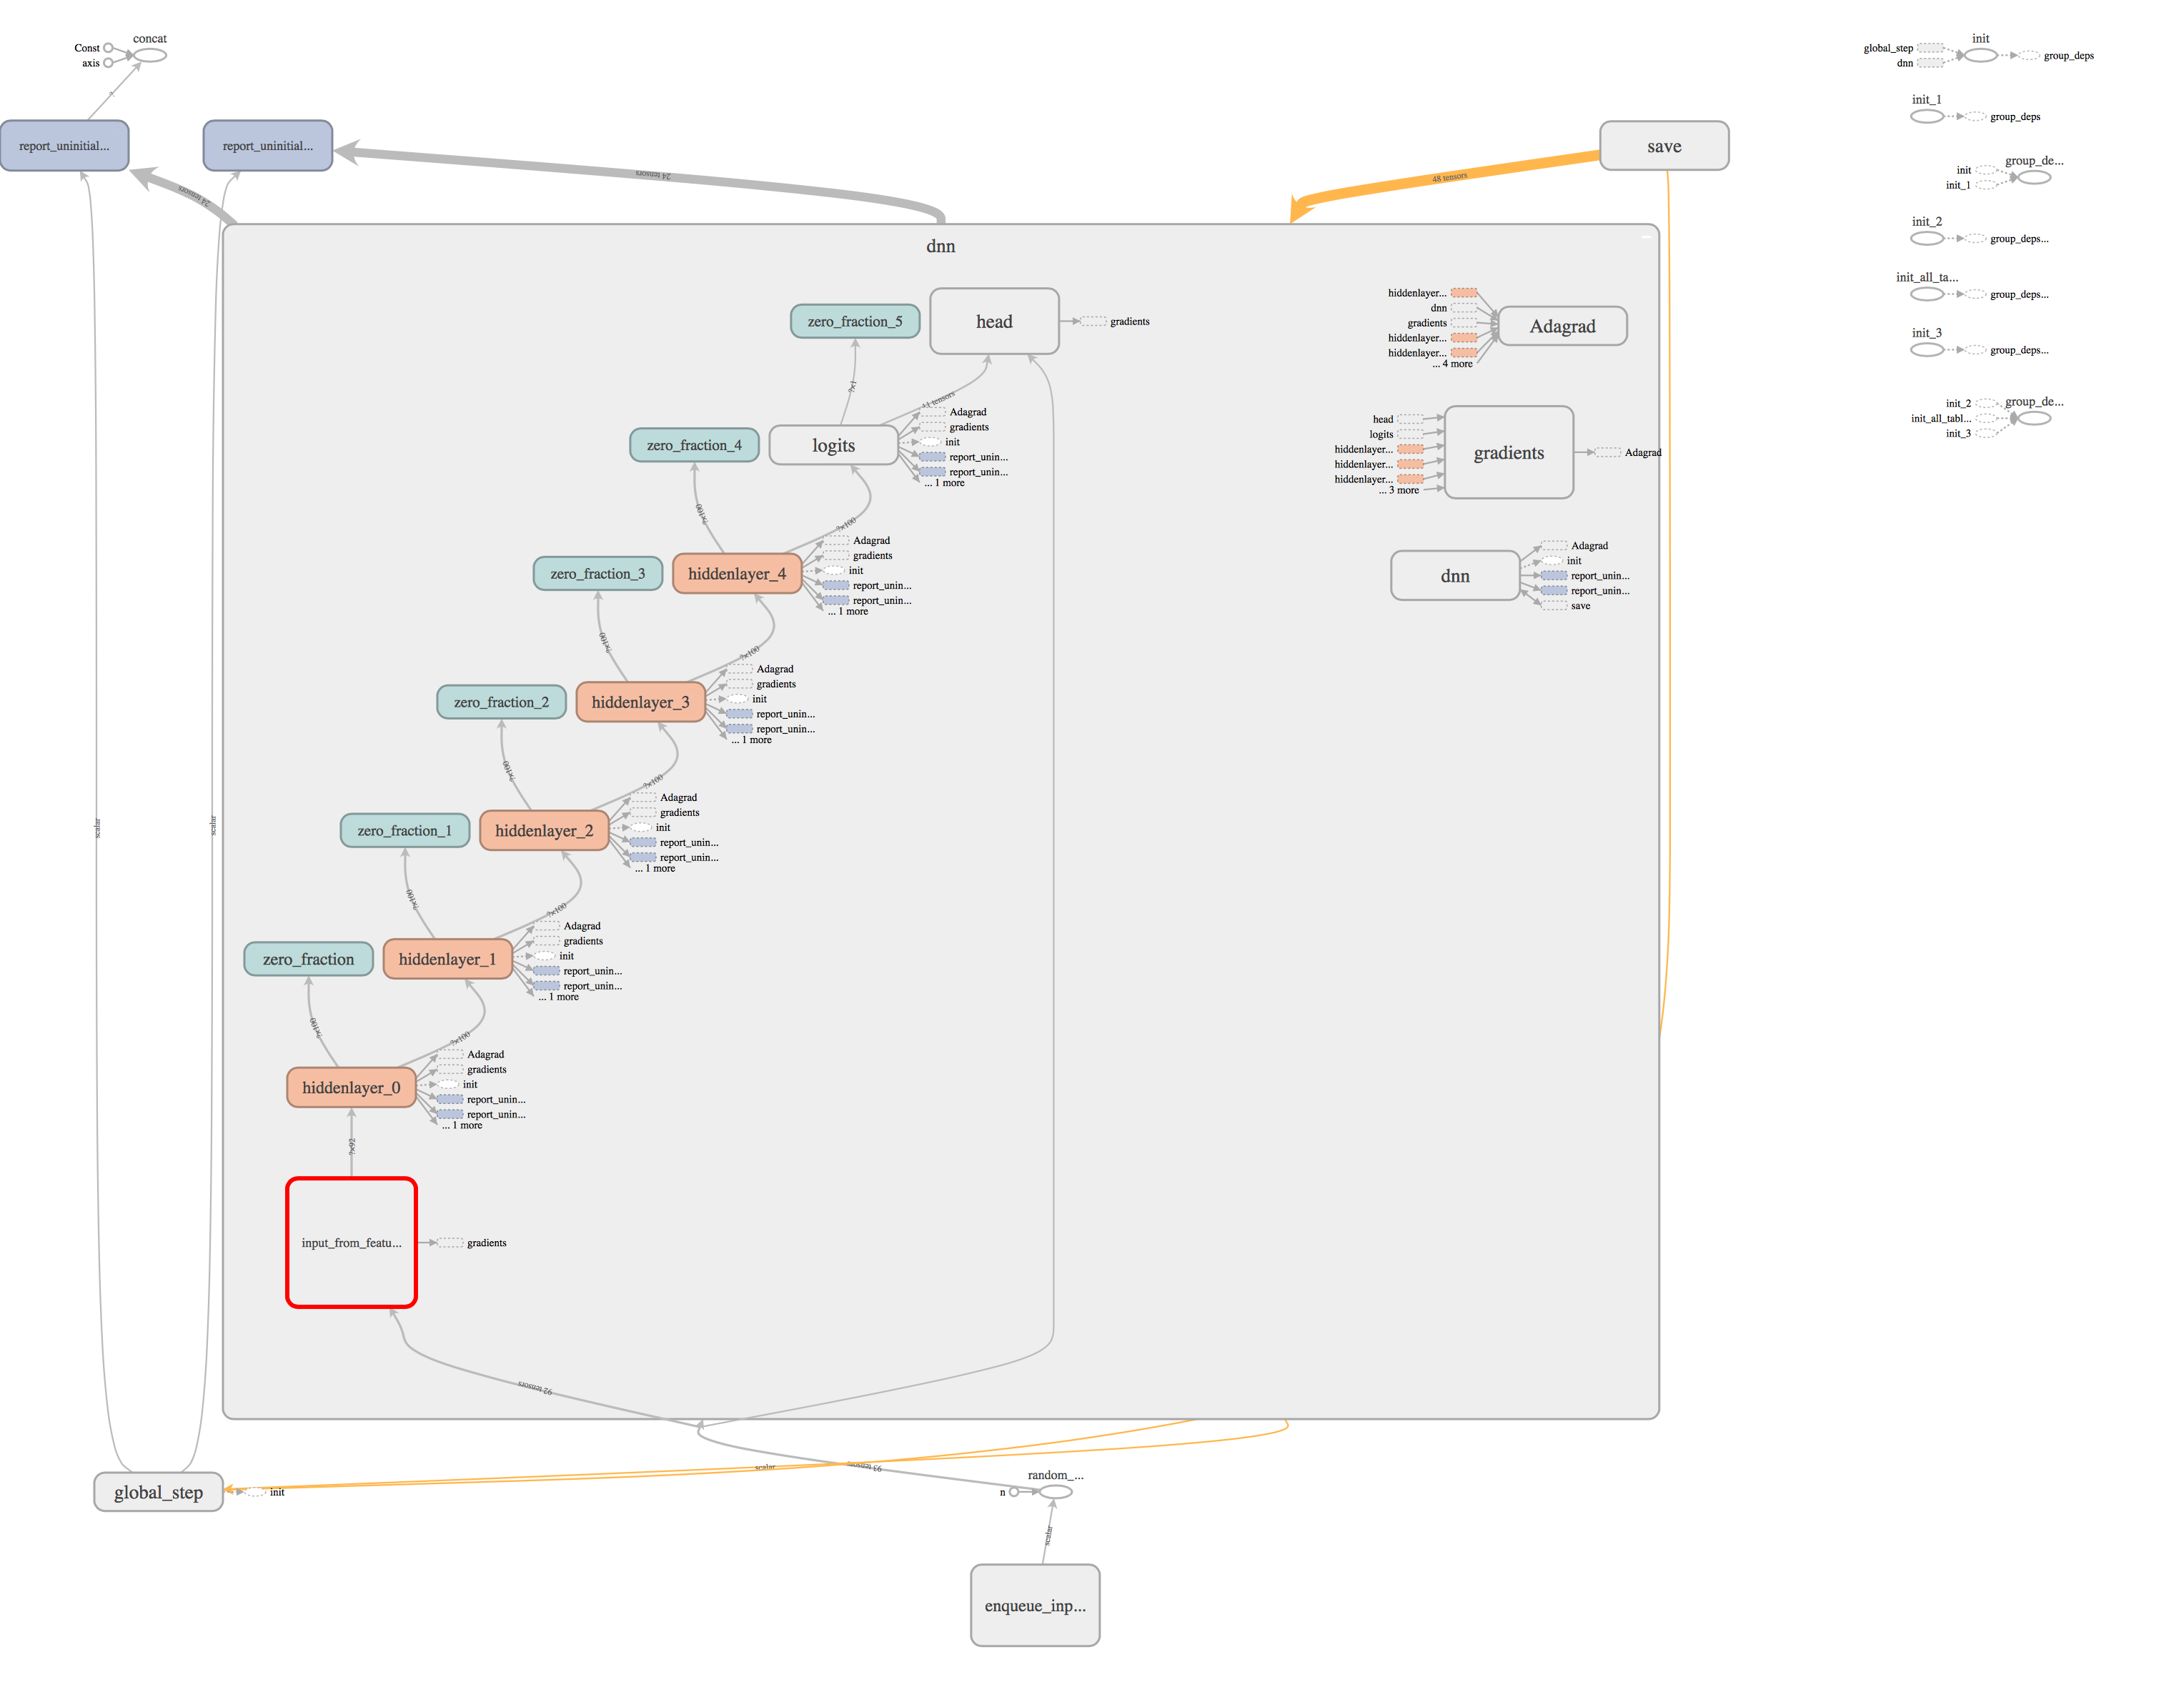
\includegraphics[width=0.9\textwidth]{diagrams/binary_class_network_diagram.png}
             \caption{Network Graph - Source: TensorBoard}
        \end{center}
        \end{figure}
    \end{columns}
\end{frame}

\begin{frame}
    \frametitle{DNN - Binary Classification}
    \begin{columns}
      \column{0.5\linewidth}
        \begin{itemize}
            \item{Selecting the best feature set}
            \item{Primary metric: accuracy}
            \item{Aim for lower loss, caveat: overfitting}
            \item{Key:}
            \begin{itemize}
              \item{\textbf{usr}: User CPU}
              \item{\textbf{used}: Used Memory}
              \item{\textbf{1m}: System Load - 1min Average}
              \item{Data Resolution: \textbf{1min}}
              \item{Source: TensorFlow evaluation}
            \end{itemize}
            \item{Winner: (\textbf{usr}, \textbf{1m}) tuple}
            \item{Accuracy achieved: \emph{\textbf{0.992}}}
            \item{6 mistakes on a 791 test set}
        \end{itemize}
      \column{0.5\linewidth}
        \begin{center}
        \begin{figure}
          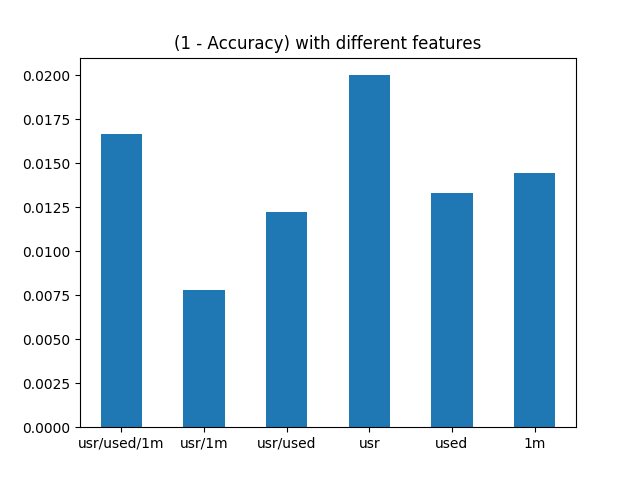
\includegraphics[width=0.8\textwidth,height=0.4\textheight]{graphs/accuracy_by_feature-status.png}
        \end{figure}
        \begin{figure}
          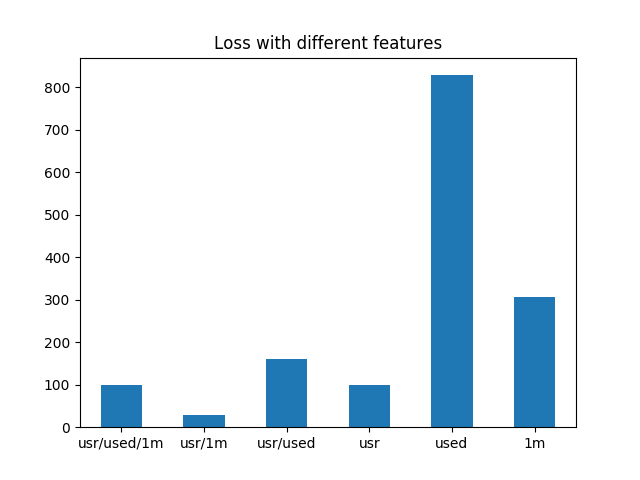
\includegraphics[width=0.8\textwidth,height=0.4\textheight]{graphs/loss_by_feature-status.png}
        \end{figure}
        % NOTE: check how total loss is calculated.
      \end{center}
  \end{columns}
\end{frame}

\begin{frame}
    \frametitle{DNN - Binary Classification}
    \begin{columns}
      \column{0.5\linewidth}
        \begin{itemize}
            \item{Selecting the data resolution}
            \item{Primary metric: accuracy}
            \item{Aim for lower loss, caveat: overfitting}
            \item{Note: careful with NaN after down-sampling}
            % On a pandas dataset, out.dropna() to remove any NaN. We cannot trust data to be 100% clean all the time, if there are missing sample they may cause NaN
            \item{Key:}
            \begin{itemize}
              \item{Original data frequency: 1s}
              \item{x-axis: new sampling rate}
              \item{Features: (\textbf{usr}, \textbf{1m})}
              \item{Source: TensorFlow evaluation}
            \end{itemize}
            \item{Winner: \textbf{10s}}
            \item{Accuracy achieved: \emph{\textbf{0.993}}}
            \item{6 mistakes on a 791 test set}
        \end{itemize}
      \column{0.5\linewidth}
        \begin{center}
        \begin{figure}
          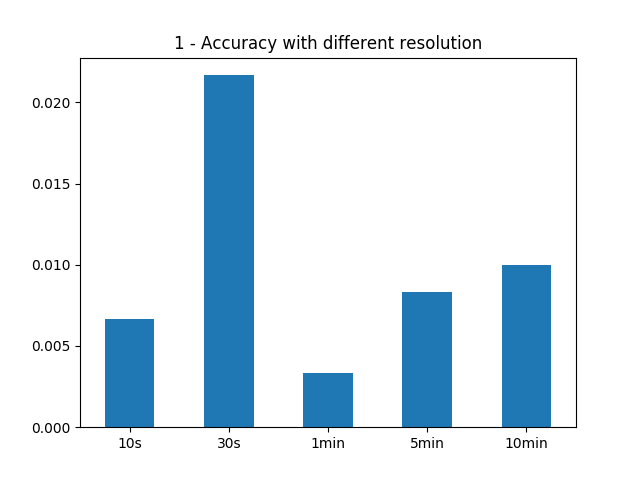
\includegraphics[width=0.8\textwidth,height=0.4\textheight]{graphs/accuracy_by_sampling-status.png}
        \end{figure}
        \begin{figure}
          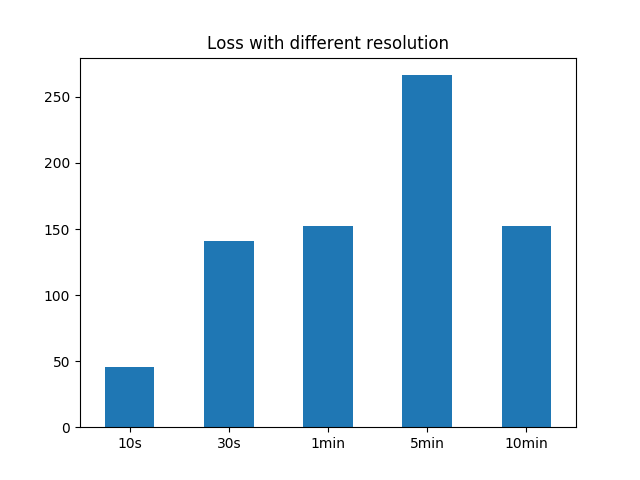
\includegraphics[width=0.8\textwidth,height=0.4\textheight]{graphs/loss_by_sampling-status.png}
        \end{figure}
      \end{center}
  \end{columns}
\end{frame}

\begin{frame}
    \frametitle{DNN - Binary Classification - Metrics report}
    \begin{columns}
      \column{0.5\linewidth}
%Add metric report for usr,1m,1min and usr,1m,10s
      \begin{table}[h!]
        \begin{center}
          \caption{Metrics report for usr\,1m and 1min}
          %\label{Metrics report for usr_1m-10s}
          \resizebox{0.6\linewidth}{!}{
            \pgfplotstabletypeset[
              every head row/.style={after row=\midrule},
              columns/status/.style={string type},
              every row no 1/.style={after row=\midrule},
            ]{code/metrics_report_binary_1min.csv}
          }
        \end{center}
      \end{table}

      \begin{figure}
        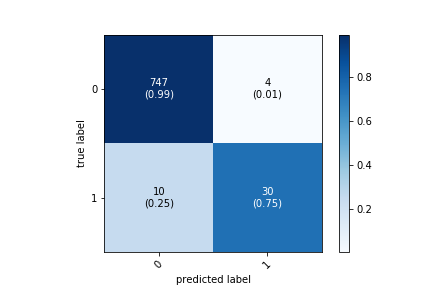
\includegraphics[width=0.8\textwidth,height=0.4\textheight]{graphs/confusion_plots/usr_1m-1min-statusdnn-5x100-500epochs-bs128.png}
      \end{figure}
      \column{0.5\linewidth}
      \begin{table}[h!]
        \begin{center}
          \caption{Metrics report for usr\,1m and 10s}
      %    \label{unrolled_sample}
          \resizebox{0.6\linewidth}{!}{
            \pgfplotstabletypeset[
              every head row/.style={after row=\midrule},
              columns/status/.style={string type},
              every row no 1/.style={after row=\midrule},
              ]{code/metrics_report_binary_10s.csv}
          }
      \end{center}
      \end{table}
        \begin{center}
          \begin{figure}
            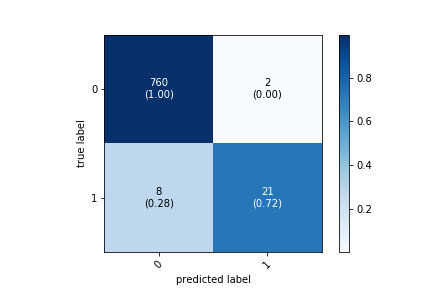
\includegraphics[width=0.8\textwidth,height=0.4\textheight]{graphs/confusion_plots/usr_1m-10s-statusdnn-5x100-500epochs-bs128.png}
          \end{figure}
        \end{center}
  \end{columns}
\end{frame}

\begin{frame}
    \frametitle{Changing test job}
    \begin{columns}
      \column{0.5\linewidth}
        \begin{table}[h!]
          \begin{center}
            \label{binary_eval_compare}
            % Update accuracy to match previous slides
            \resizebox{1\linewidth}{!}{
              \pgfplotstabletypeset[
                precision=3,
                columns/metric/.style={string type},
                every head row/.style={after row=\midrule},
                every even row={5}{before row=\rowcolor{mygray}},
              ]{code/usr_1m-10s-status-eval-compare.csv}
            }
          \end{center}
       \end{table}
      \column{0.5\linewidth}
        \begin{itemize}
            \item{Train with "tempest-full"}
            \item{Evaluating with "tempest-full-py3"}
            \begin{itemize}
              \item{Similar setup, uses python3}
              \item{It does not include swift and swift tests}
              \item{600 examples evaluation set}
            \end{itemize}
            \item{Dataset and training setup:}
            \begin{itemize}
              \item{Features: (usr, 1m)}
              \item{Resolution: 1min}
              \item{Same hyper-parameters}
            \end{itemize}
        \end{itemize}
    \end{columns}
\end{frame}

\begin{frame}
    \frametitle{Binary Classification - Summary}
    \begin{columns}
      \column{0.4\linewidth}
        \begin{itemize}
            \item{Features: User CPU and 1min Load Avg}
            \item{Resolution: 10s best, 1 minute may be enough}
            \item{High accuracy: \emph{\textbf{0.993}}}
            \item{High precision, recall and F1-score}
            \item{A trained model might be applicable to similar CI jobs}
        \end{itemize}
      \column{0.6\linewidth}
        \begin{figure}
          \begin{center}
            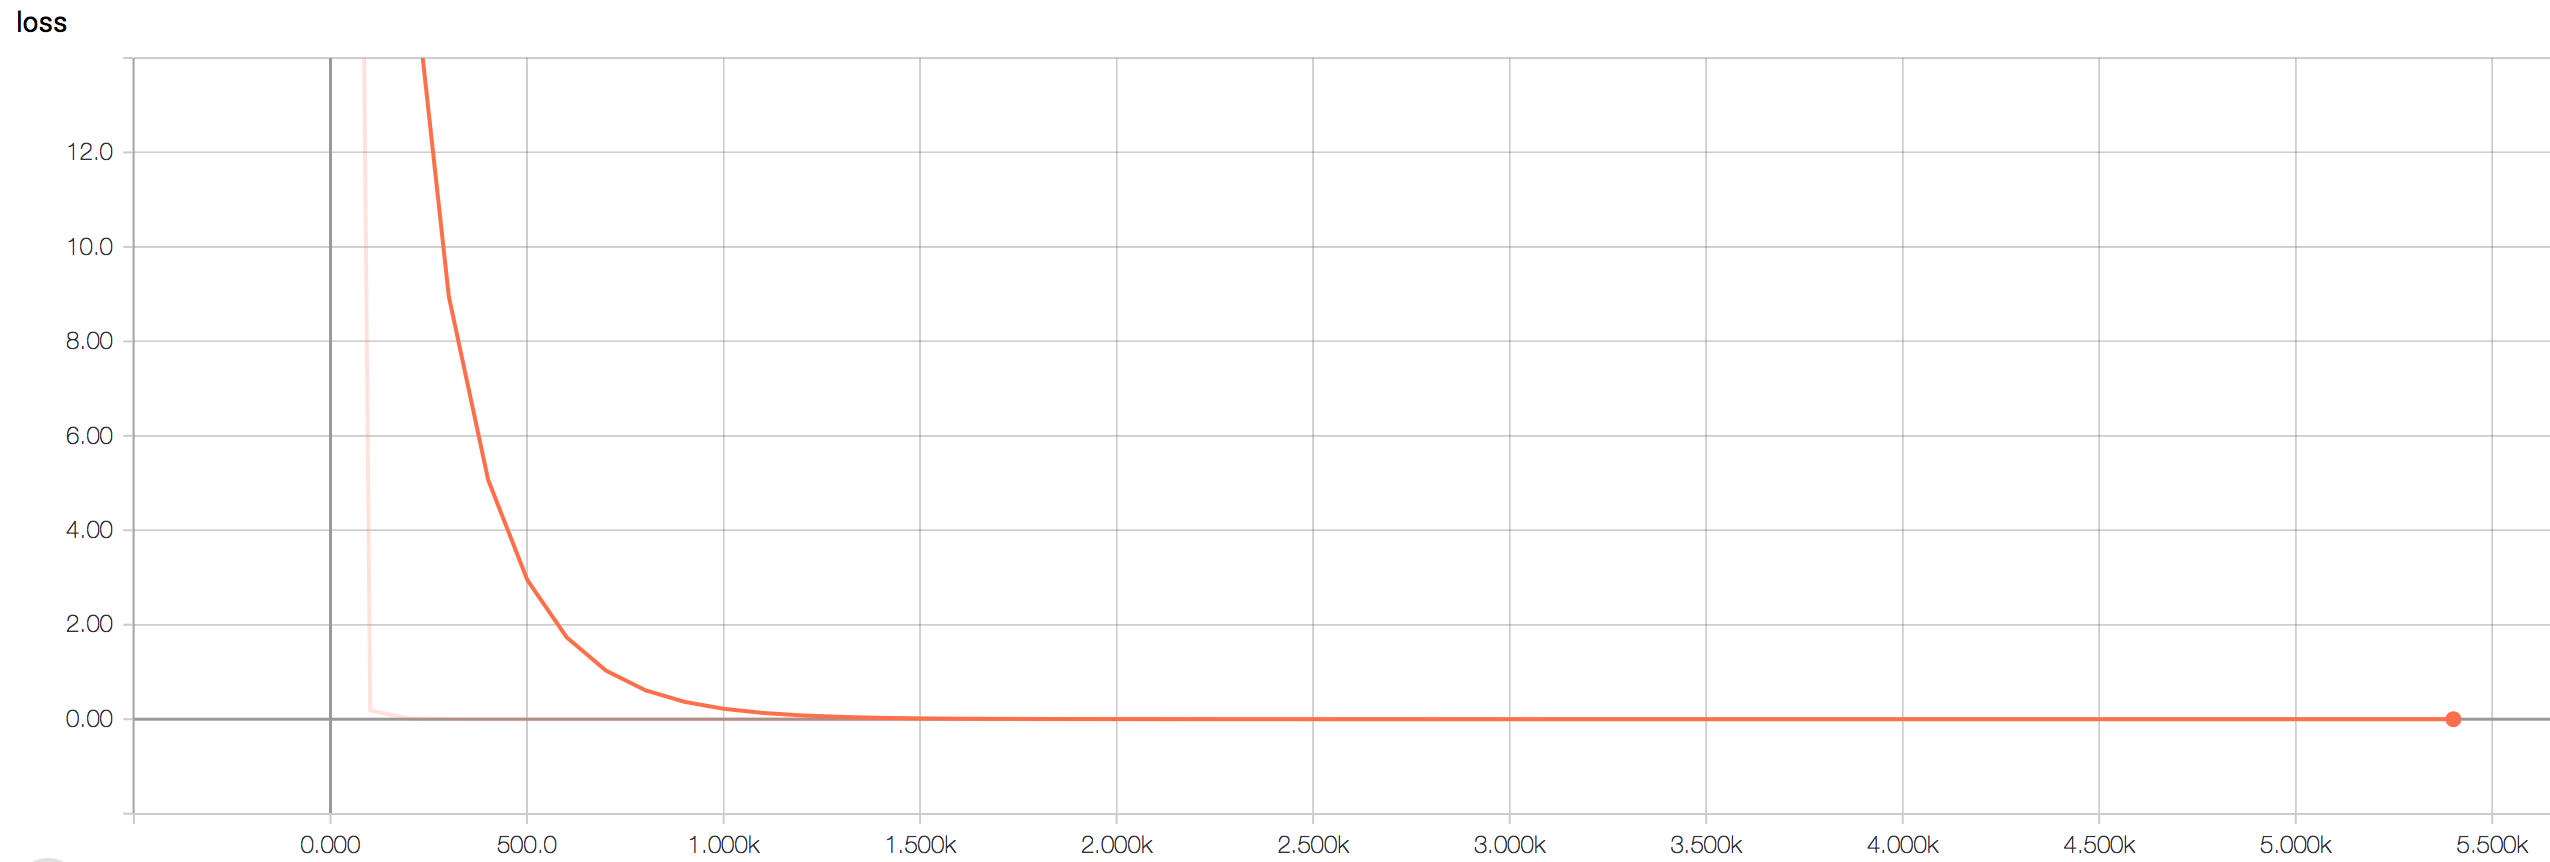
\includegraphics[width=0.9\textwidth,height=0.5\textheight]{graphs/cpu_1m-1min-status_loss_curve.png}
              \caption{Training Loss - usr/1m, 1min - Source: TensorBoard}
          \end{center}
        \end{figure}
      \end{columns}
\end{frame}

\begin{frame}
    \frametitle{DNN - Multi Class}
    \begin{columns}
      \column{0.5\linewidth}
        \begin{itemize}
            \item{Classes: Hosting Cloud Provider}
            \item{Supervised training}
            \item{TensorFlow \emph{DNNClassifier}, classes=\textbf{10}}
            \item{Dataset:}
            \begin{itemize}
              \item{CI Job "tempest-full"}
              \item{Gate pipeline only}
              \item{3000 examples, 2100 training, 900 test}
            \end{itemize}
            \item{Hyper-parameters:}
            \begin{itemize}
              \item{Activation function: ReLU}
              \item{Output layer: Sigmoid}
              \item{Optimizer: Adagrad}
              \item{Learning rate (initial): 0.05}
              \item{5 hidden layers, 100 units per layer}
              \item{Batch Size: 128, Epochs: 500}
            \end{itemize}
        \end{itemize}
      \column{0.5\linewidth}
        \begin{figure}
        \begin{center}
          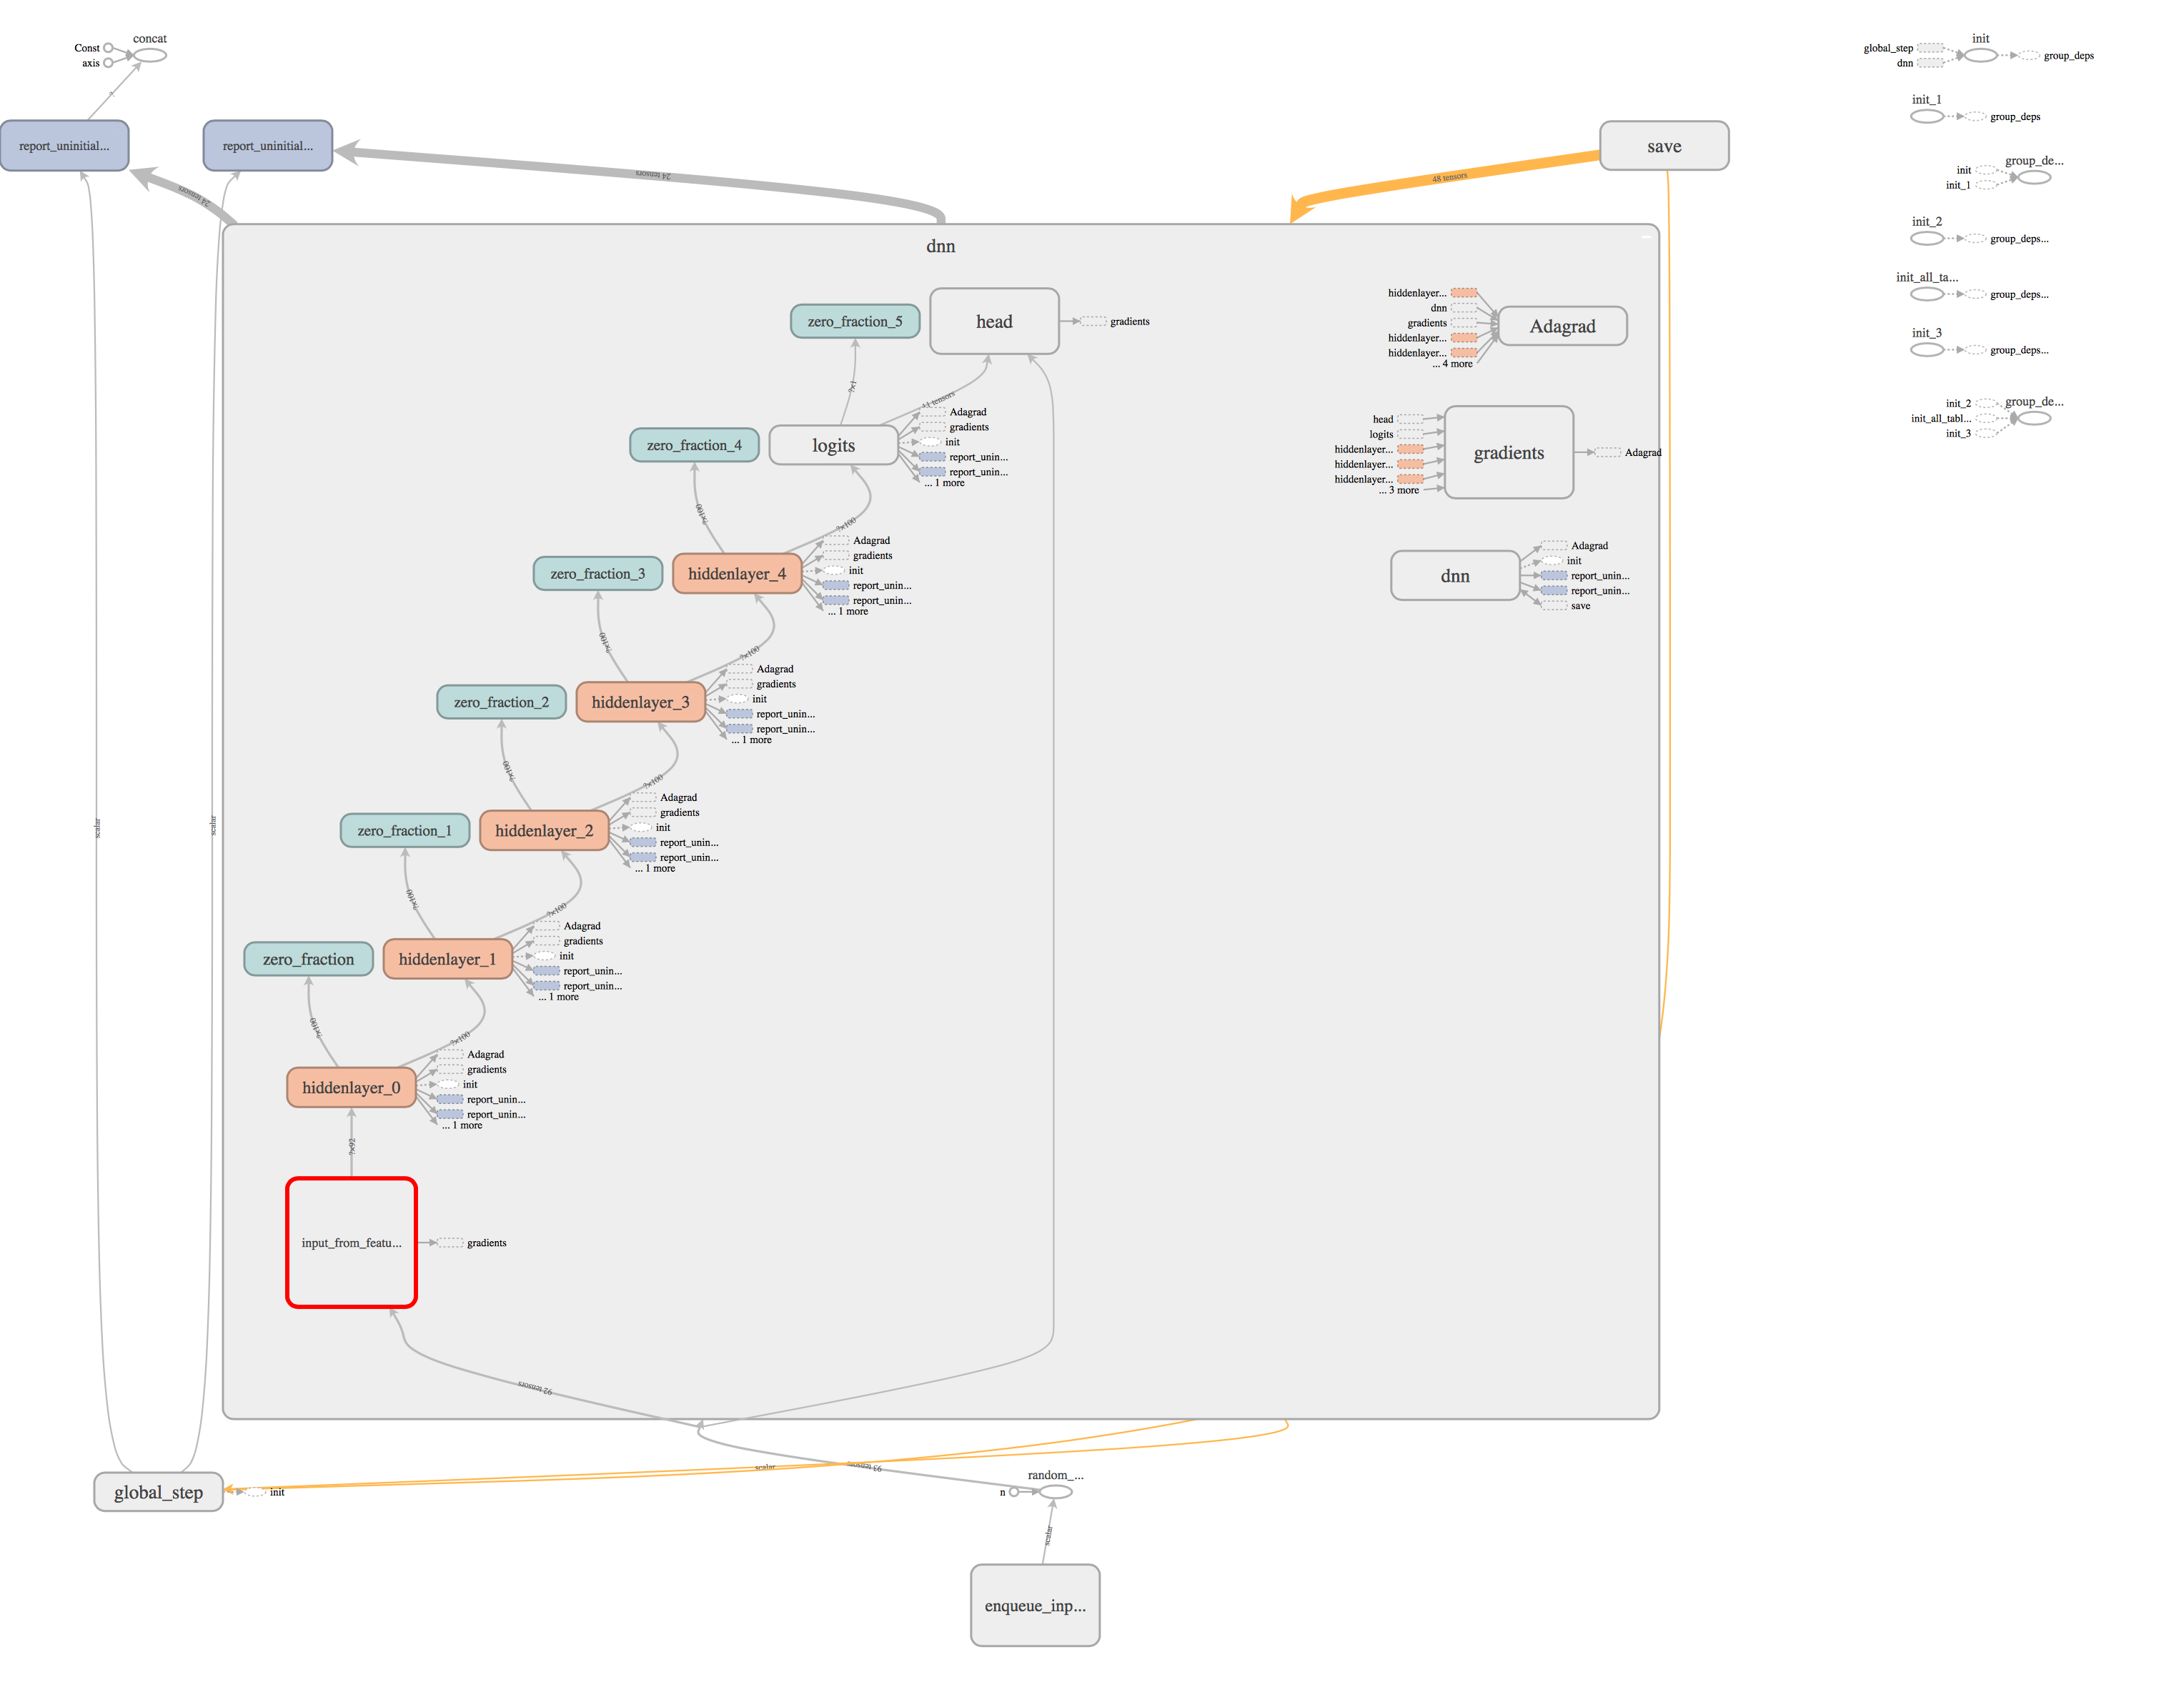
\includegraphics[width=0.9\textwidth]{diagrams/binary_class_network_diagram.png}
             \caption{Network Graph - Source: TensorBoard}
        \end{center}
        \end{figure}
    \end{columns}
\end{frame}

\begin{frame}
    \frametitle{DNN - Multi Class}
    \begin{columns}
      \column{0.4\linewidth}
        \begin{itemize}
          \item{Features: (usr, 1m)}
          \item{Resolution: 1min}
          \item{Loss converges, but...}
          \item{Evaluation accuracy achieved: \emph{\textbf{0.601}}}
          \item{Not good!}
        \end{itemize}
      \column{0.6\linewidth}
        \begin{figure}
          \begin{center}
            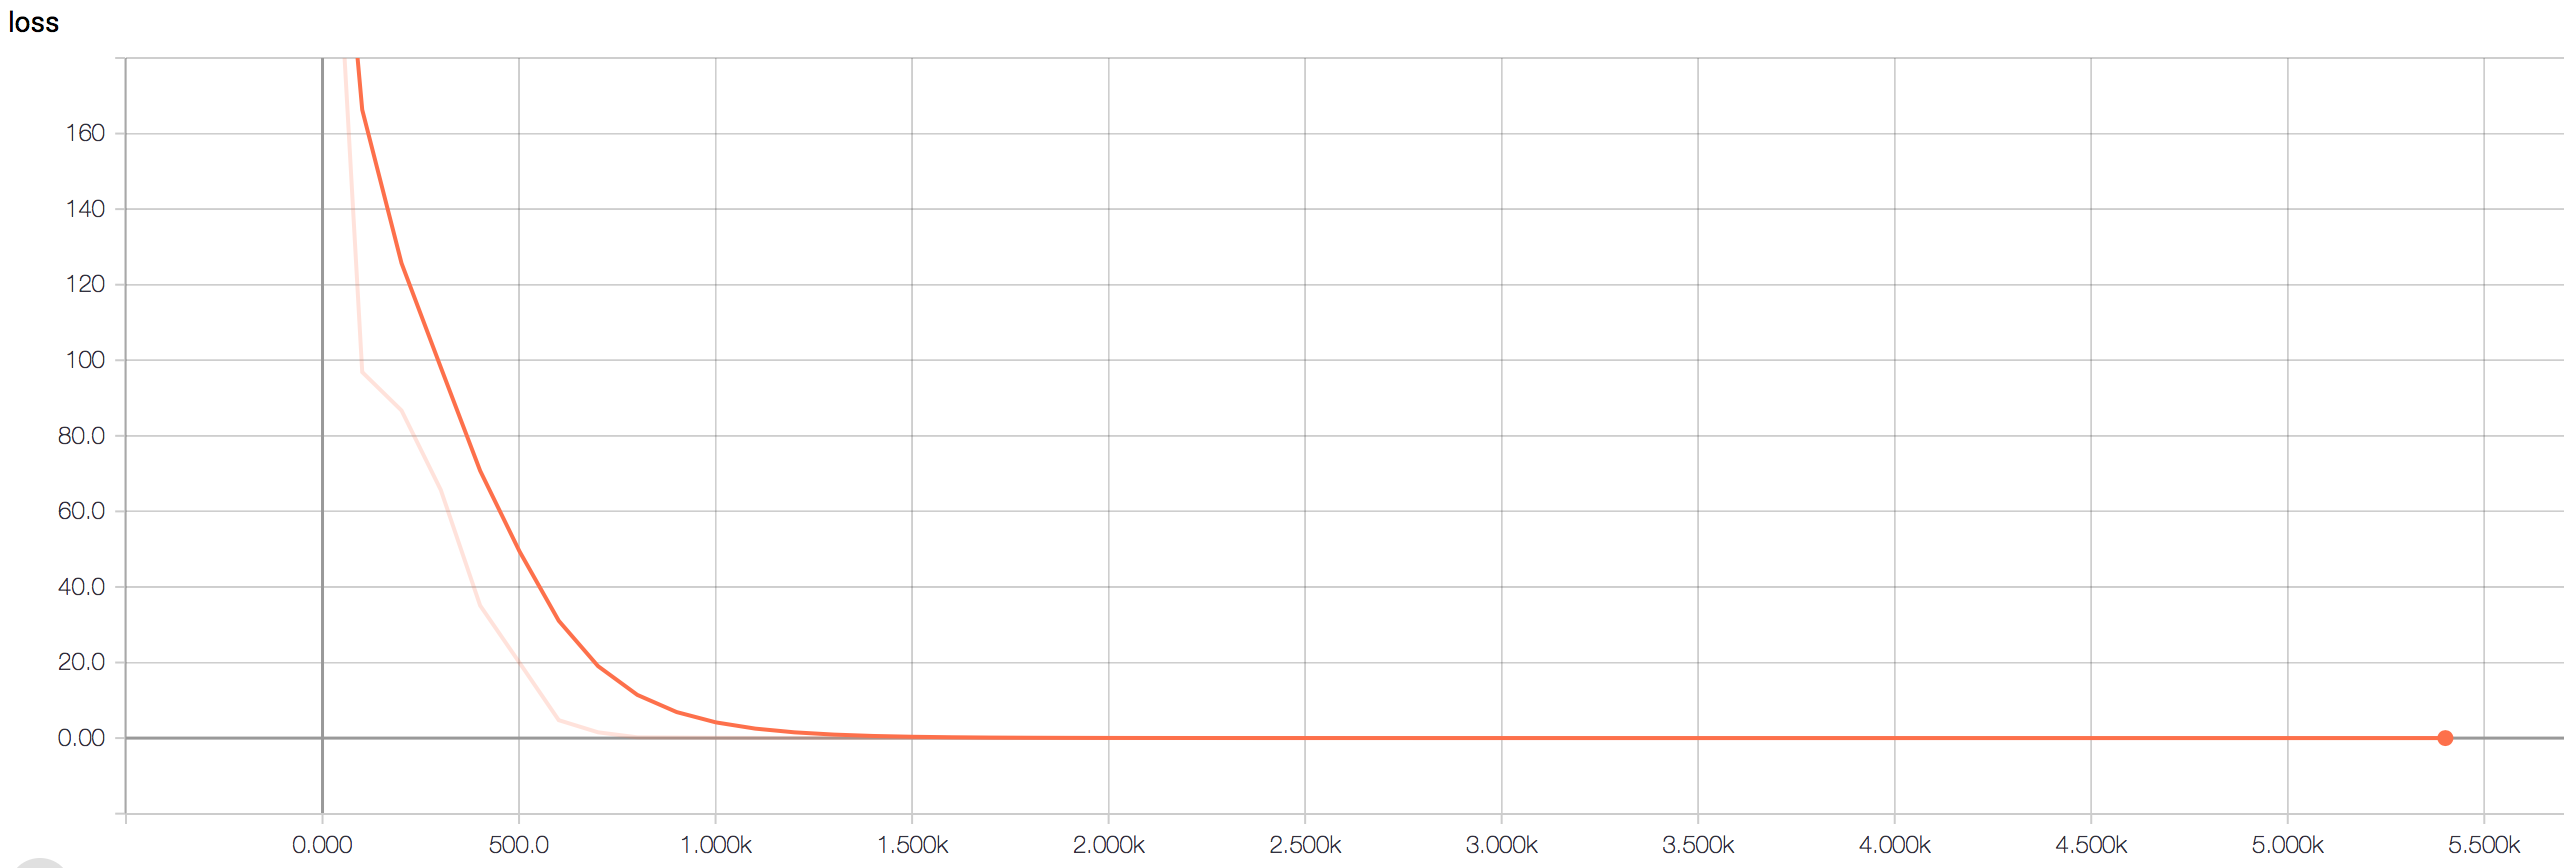
\includegraphics[width=0.9\textwidth,height=0.5\textheight]{graphs/cpu_1m-1min-node_provider_all_loss_curve.png}
              \caption{Training Loss - usr/1m, 1min - Source: TensorBoard}
          \end{center}
        \end{figure}
      \end{columns}
\end{frame}

\begin{frame}
    \frametitle{Multi Class - Different Features}
    \begin{columns}
      \column{0.5\linewidth}
        \begin{itemize}
            \item{Try different combinations of features}
            \item{Primary metric: accuracy}
            \item{Aim for lower loss, caveat: overfitting}
            \item{Key:}
            \begin{itemize}
              \item{\textbf{usr}: User CPU}
              \item{\textbf{used}: Used Memory}
              \item{\textbf{1m}: System Load - 1min Average}
              \item{Data Resolution: \textbf{1min}}
              \item{Source: TensorFlow evaluation output}
            \end{itemize}
            \item{No real improvement}
            \item{Best accuracy achieved: \emph{\textbf{0.603}}}
            \item{Adding Disk I/O or process data does not help either}
        \end{itemize}
      \column{0.5\linewidth}
        \begin{center}
        \begin{figure}
          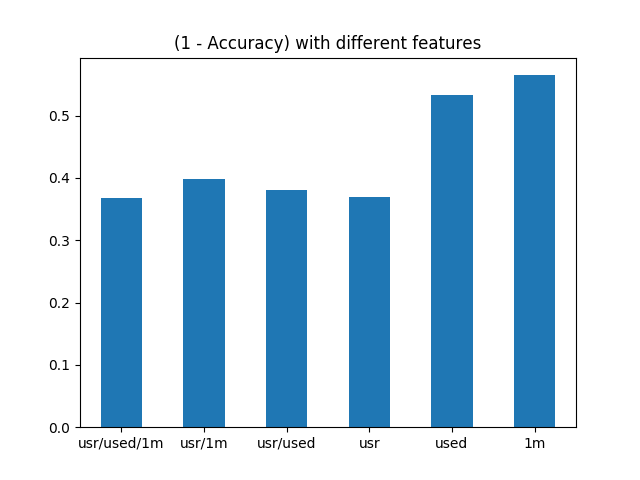
\includegraphics[width=0.8\textwidth,height=0.4\textheight]{graphs/accuracy_by_feature-node_provider_all.png}
        \end{figure}
        \begin{figure}
          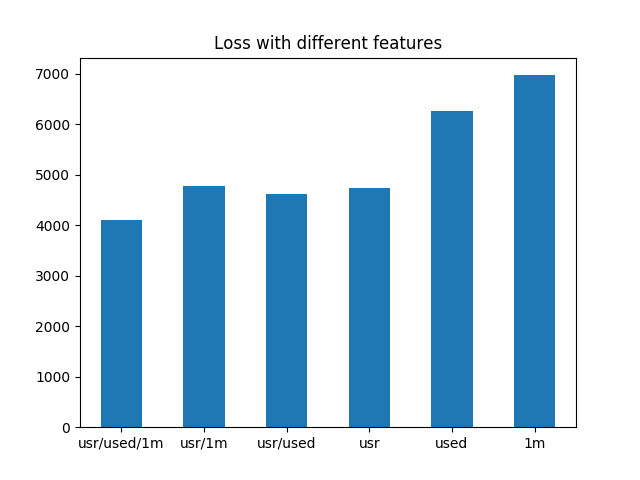
\includegraphics[width=0.8\textwidth,height=0.4\textheight]{graphs/loss_by_feature-node_provider_all.png}
        \end{figure}
      \end{center}
  \end{columns}
\end{frame}

\begin{frame}
    \frametitle{Multi Class - Changing Resolution}
    \begin{columns}
      \column{0.5\linewidth}
        \begin{itemize}
            \item{Trying to change the data resolution}
            \item{Primary metric: accuracy}
            \item{Aim for lower loss, caveat: overfitting}
            \item{Key:}
            \begin{itemize}
              \item{Original data frequency: 1s}
              \item{x-axis: new sampling rate}
              \item{Features: (\textbf{usr}, \textbf{1m})}
              \item{Source: TensorFlow evaluation}
            \end{itemize}
            \item{No real improvement}
            \item{Best accuracy achieved: \emph{\textbf{0.624}}}
        \end{itemize}
      \column{0.5\linewidth}
        \begin{center}
        \begin{figure}
          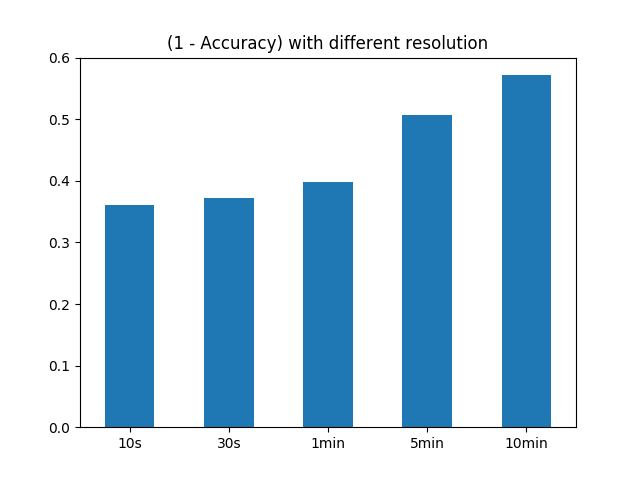
\includegraphics[width=0.8\textwidth,height=0.4\textheight]{graphs/accuracy_by_sampling-node_provider_all.png}
        \end{figure}
        \begin{figure}
          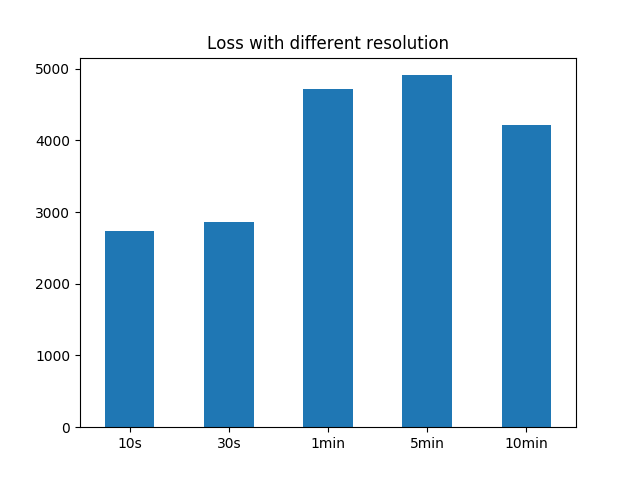
\includegraphics[width=0.8\textwidth,height=0.4\textheight]{graphs/loss_by_sampling-node_provider_all.png}
        \end{figure}
      \end{center}
  \end{columns}
\end{frame}

\begin{frame}
    \frametitle{Multi Class - Network topology}
    \begin{columns}
      \column{0.5\linewidth}
        \begin{itemize}
            \item{Trying to change the network depth}
            \item{Trying to change number of units per layer}
            \item{Primary metric: accuracy}
            \item{Aim for lower loss, caveat: overfitting}
            \item{Key:}
            \begin{itemize}
              \item{x-axis: units and hidden layers}
              \item{Features: (\textbf{usr}, \textbf{1m})}
              \item{Resolution: \textbf{1min}}
              \item{Source: TensorFlow evaluation}
            \end{itemize}
            \item{No real improvement}
            \item{Best accuracy achieved: \emph{\textbf{0.668}}}
        \end{itemize}
      \column{0.5\linewidth}
        \begin{center}
        \begin{figure}
          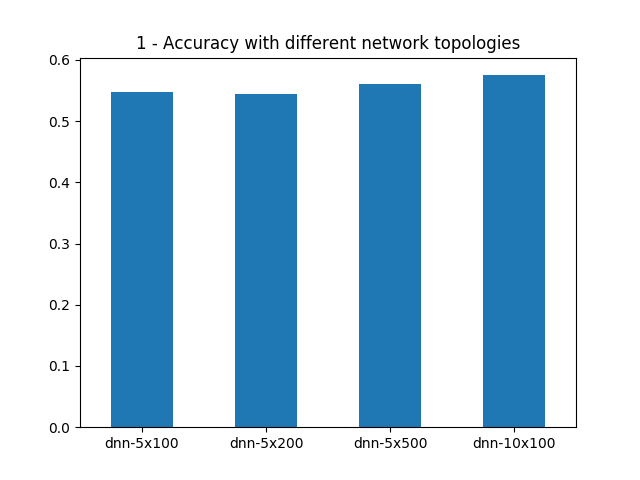
\includegraphics[width=0.8\textwidth,height=0.4\textheight]{graphs/accuracy_by_topology-node_provider_all.png}
        \end{figure}
        \begin{figure}
          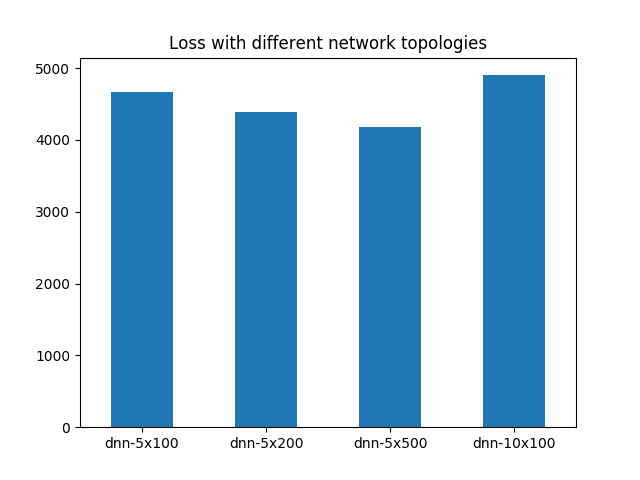
\includegraphics[width=0.8\textwidth,height=0.4\textheight]{graphs/loss_by_topology-node_provider_all.png}
        \end{figure}
      \end{center}
  \end{columns}
\end{frame}

\begin{frame}
    \frametitle{Multi Class - Reducing the number of classes}
    \begin{columns}
      \column{0.5\linewidth}
        \begin{itemize}
            \item{Reducing the number of classes}
            \begin{itemize}
                \item{Different regions from a Cloud Operator}
                \item{Consider as a single class}
                \item{New number of classes is \textbf{7}}
            \end{itemize}
            \item{Experiments:}
              \begin{itemize}
                \item{Train with different feature sets}
                \item{Train with different resolutions}
                \item{Source: TensorFlow evaluation}
            \end{itemize}
            \item{Significant improvement!}
            \item{Best accuracy achieved: \emph{\textbf{0.902}}}
            \item{What does that mean?}
        \end{itemize}
      \column{0.5\linewidth}
        \begin{center}
        \begin{figure}
          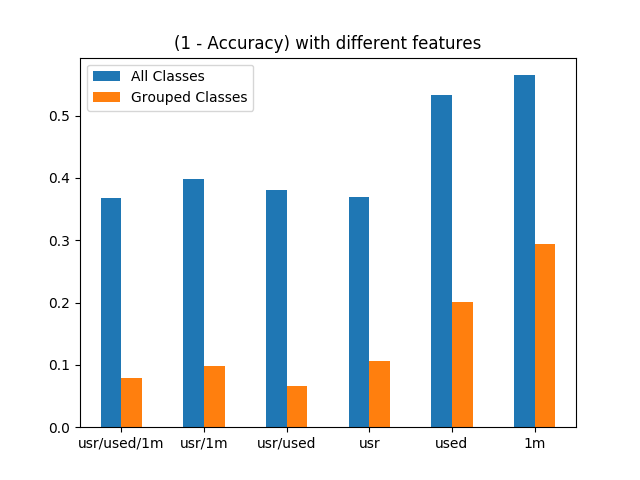
\includegraphics[width=0.8\textwidth,height=0.4\textheight]{graphs/accuracy_by_feature-compare-classes.png}
        \end{figure}
        \begin{figure}
          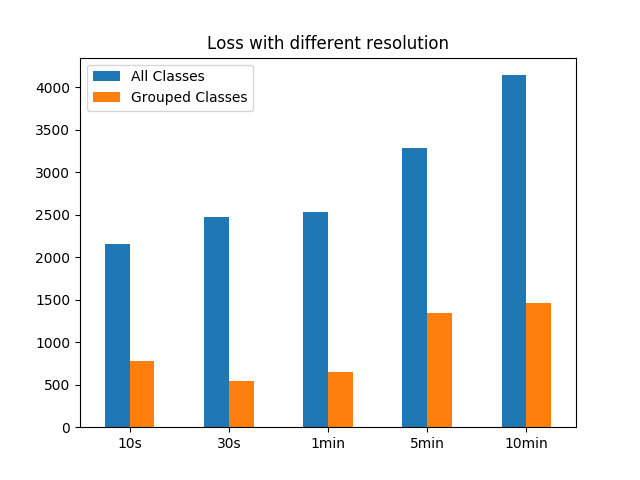
\includegraphics[width=0.8\textwidth,height=0.4\textheight]{graphs/loss_by_sampling-compare-classes.png}
        \end{figure}
        \end{center}
  \end{columns}
\end{frame}

\begin{frame}
    \frametitle{Multi Class - Tuning network topology}
    \begin{columns}
      \column{0.5\linewidth}
        \begin{itemize}
            \item{Tuning network topology}
            \item{Experiments:}
            \begin{itemize}
              \item{x-axis: units and hidden layers}
              \item{Features: (\textbf{usr}, \textbf{1m})}
              \item{Resolution: \textbf{1min}}
            \end{itemize}
            \item{Some improvement}
            \item{Winner: 3x100. Accuracy: \emph{\textbf{0.925}}}
        \end{itemize}
      \column{0.5\linewidth}
        \begin{center}
        \begin{figure}
          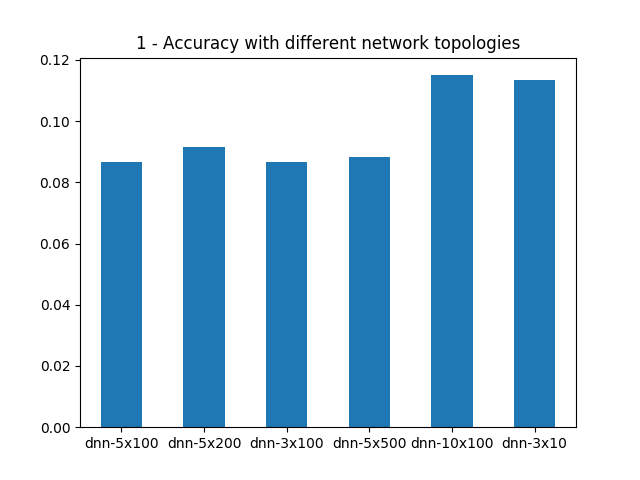
\includegraphics[width=0.8\textwidth,height=0.4\textheight]{graphs/accuracy_by_topology-node_provider.png}
        \end{figure}
        \begin{figure}
          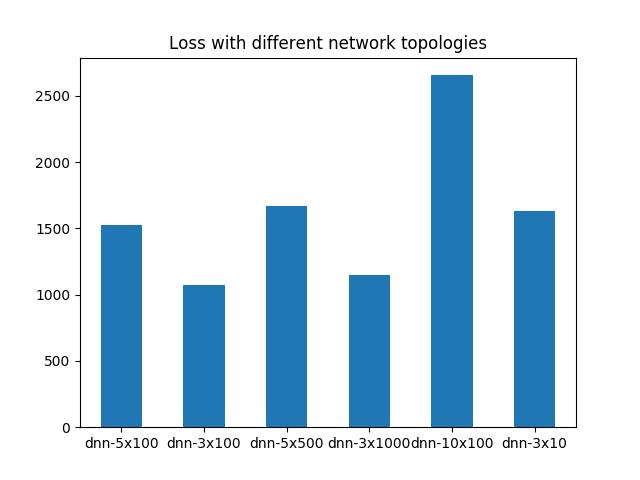
\includegraphics[width=0.8\textwidth,height=0.4\textheight]{graphs/loss_by_topology-node_provider.png}
        \end{figure}
        \end{center}
  \end{columns}
\end{frame}

\begin{frame}
    \frametitle{Multi Class - Metrics report}
    \begin{columns}
      \column{0.5\linewidth}
        \begin{itemize}
            \item{Experiment:}
            \begin{itemize}
              \item{Dataset: 3955 examples split in 60\% training, 20\% dev and 20\% test}
              \item{Features: User CPU and Load Avg}
              \item{Resolution: 1 minute}
              \item{Hyperparameters: 3 hidden layers, 1000 units each}
              \item{Cloud providers: 7}
            \end{itemize}
        \end{itemize}
        \begin{center}
         \begin{table}[h!]
           \caption{Metrics report for usr\,1m and 1min}
       %    \label{unrolled_sample}
           \resizebox{0.6\linewidth}{!}{
             \pgfplotstabletypeset[
               every head row/.style={after row=\midrule},
               columns/provider/.style={string type},
               every row no 6/.style={after row=\midrule},
               ]{code/metrics_report_multiclass_1min.csv}
           }
         \end{table}
        \end{center}
      \column{0.5\linewidth}
       \begin{center}
        \begin{figure}
          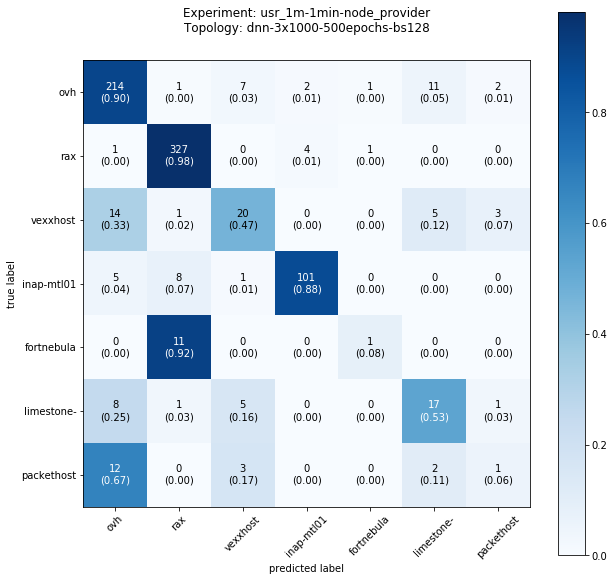
\includegraphics[width=0.85\textwidth]{graphs/confusion_plots/usr_1n_1min_3x1000_title_new.png}
        \end{figure}
        \end{center}
        \vfill
  \end{columns}
\end{frame}

\begin{frame}
    \frametitle{Multi Class - Changing test job}
    \begin{columns}
      \column{0.5\linewidth}
        \begin{table}[h!]
          \begin{center}
            \label{multi_eval_compare}
            \resizebox{1\linewidth}{!}{
              \pgfplotstabletypeset[
                precision=3,
                columns/metric/.style={string type},
                every head row/.style={after row=\midrule},
                every even row={5}{before row=\rowcolor{mygray}},
              ]{code/usr_1m-1min-node_provider-eval-compare.csv}
            }
          \end{center}
       \end{table}
      \column{0.5\linewidth}
        \begin{itemize}
            \item{Train with "tempest-full"}
            \item{Evaluating with "tempest-full-py3"}
            \begin{itemize}
              \item{Similar setup, uses python3}
              \item{It does not include swift and swift tests}
              \item{600 examples evaluation set}
            \end{itemize}
            \item{Dataset and training setup:}
            \begin{itemize}
              \item{Features: (usr, 1m)}
              \item{Resolution: 1min}
              \item{Same hyper-parameters (dnn-3x100)}
            \end{itemize}
        \end{itemize}
    \end{columns}
\end{frame}

\begin{frame}
    \frametitle{Multi Class - Summary}
    \begin{columns}
      \column{0.4\linewidth}
        \begin{itemize}
            \item{User CPU and 1min Load Avg}
            \item{Resolution: 1 minute is enough}
            \item{Hyperparameters: 3 hidden layers, 100 units each}
            \item{Reasonable accuracy: \emph{\textbf{0.925}}}
            \item{A trained model is not applicable to similar CI jobs}
        \end{itemize}
      \column{0.6\linewidth}
        \begin{figure}
          \begin{center}
            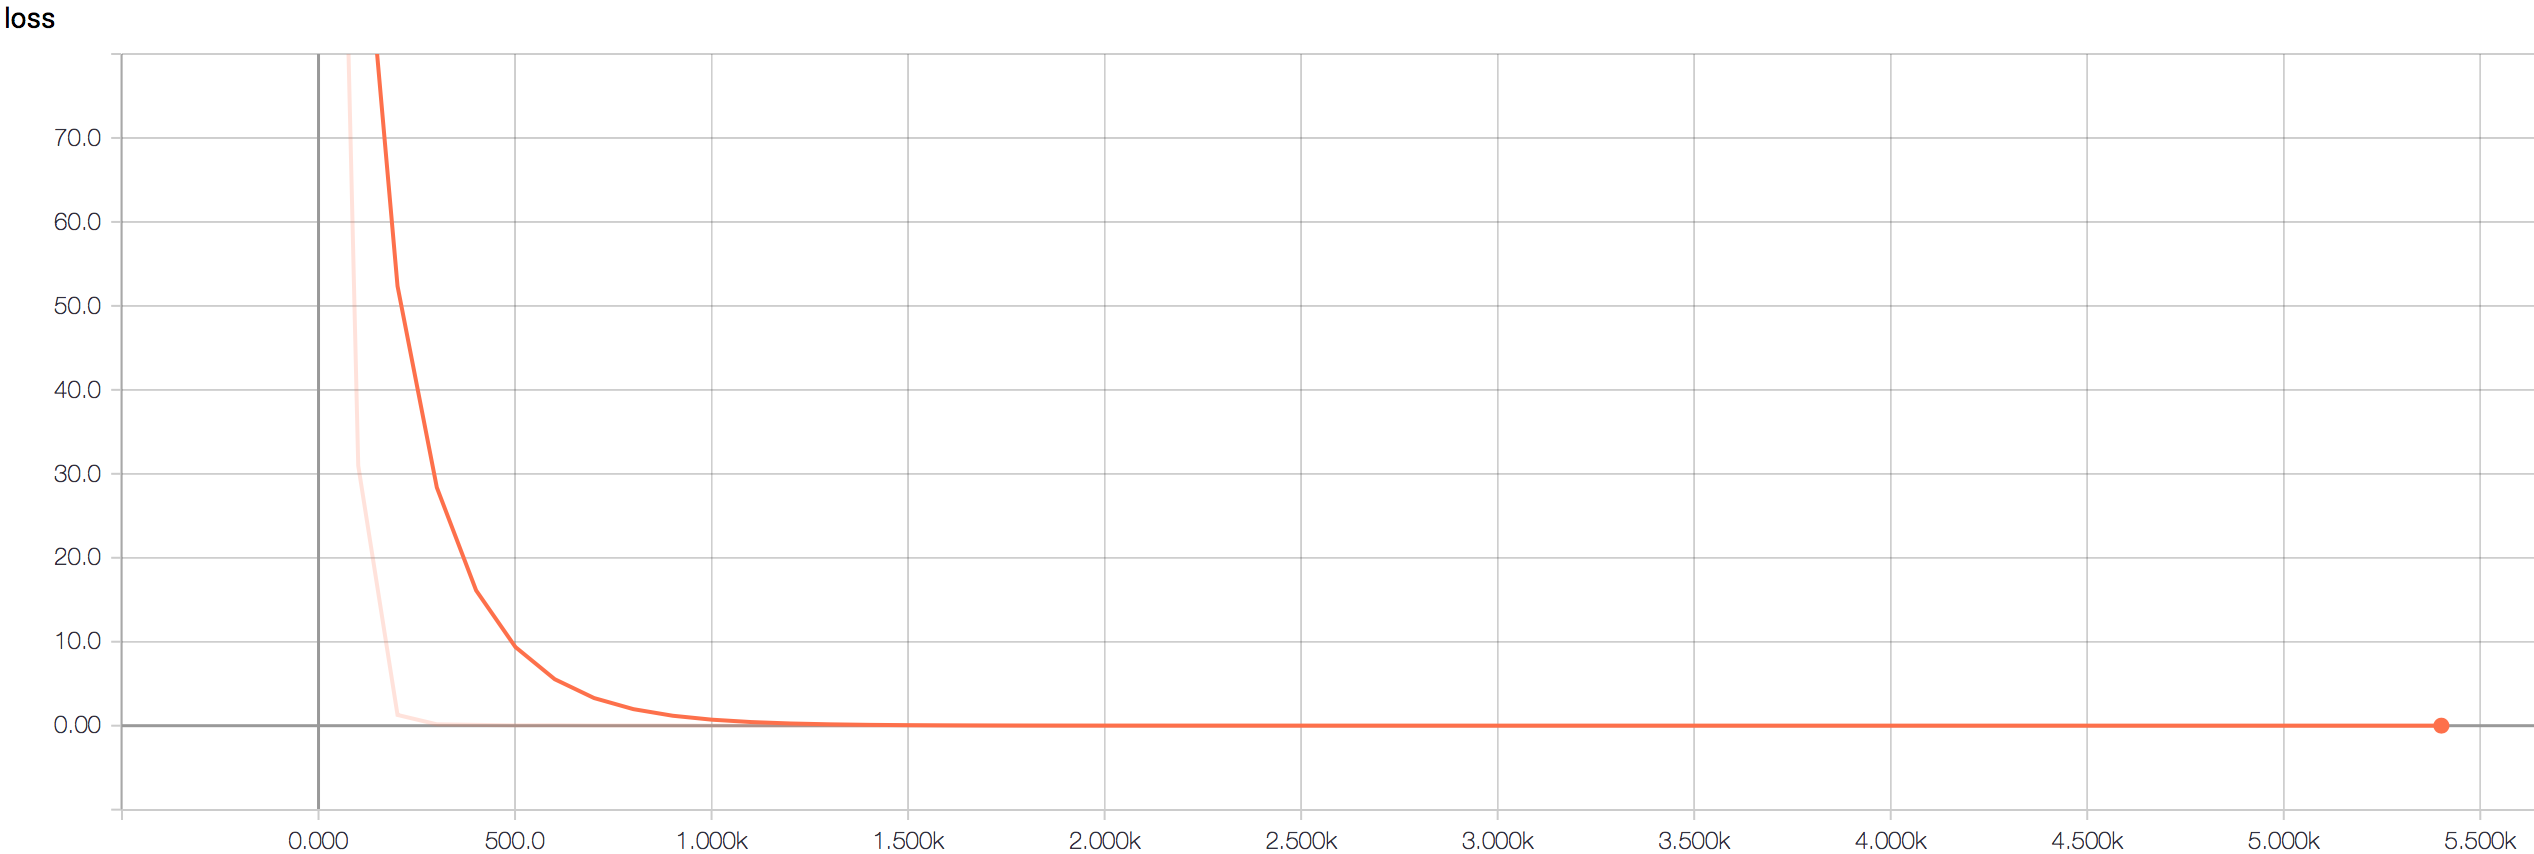
\includegraphics[width=0.9\textwidth,height=0.5\textheight]{graphs/cpu_1m-1min-dnn3x100-node_provider-loss_curve.png}
              \caption{Training Loss - usr/1m, 1min, dnn3x100 - Source: TensorBoard}
          \end{center}
        \end{figure}
      \end{columns}
\end{frame}

\section{Conclusions}
\begin{frame}
  \frametitle{Conclusions}
  \begin{itemize}
      \item{Collect data}
      \item{Know your data}
      \item{Work with cloud tools}
      \item Able to confirm that system load plays a role in failures
      \item Load profiles are consistent across regions in our cloud providers
    \end{itemize}
\end{frame}

\begin{frame}
  \frametitle{Future Work}
  \begin{itemize}
      \item{Look at adapting techniques for new models with different data}
      \item{Human curated dataset for supervised training}
      \item{Research clustering techniques for unsupervised training}
      \item{Explore job portability}
      \item{Use the pass/fail data to detect degradation in CI Jobs}
  \end{itemize}
\end{frame}

\begin{frame}
  \frametitle{Questions?}
  \begin{itemize}
      \item{This talk: \href{https://github.com/afrittoli/ciml\_talk}{https://github.com/afrittoli/ciml\_talk}}
      \item{CIML: \href{https://github.com/mtreinish/ciml}{https://github.com/mtreinish/ciml}}
  \end{itemize}
\end{frame}
\end{document}
